\documentclass{IEEEtran}
\usepackage{cite}
\usepackage{amsmath, amssymb, amsfonts}
\usepackage{algorithmic}
\usepackage{graphicx}
\usepackage{textcomp}
\usepackage{xcolor}
\usepackage{caption}
\usepackage[colorlinks=true, citecolor=., linkcolor=.]{hyperref}
\usepackage{cleveref}
\usepackage{ragged2e}
\usepackage{float}
\usepackage{setspace}
\usepackage{caption}
\usepackage{subcaption}
\begin{document}

\title{Trading Bot Optimisation}
\author{Kaiqi Liang 23344153\\Wenxiao Zhang 22792191\\Fernando Barrientos-Perez 22703003\\Isaac Bergl 22710992}
\maketitle

\section{Abstract}
This paper showcases an attempt to build on the genetic algorithm (GA) presented by MacLachlan et al. \cite{maclachlan2022genetic} by extending its use to a financial domain. We create a trading bot optimisation framework that uses the GA to refine the performance of automated trading, which is measured by the total profit.

Optuna is used to optimise the hyperparameters of the GA training regime; the number of crossovers, number of mutations, and standard deviation of change in the constant value, C, of each literal for mutation. Initial generations of GAs are seeded to allow for the fair comparison of the different hyperparameter settings. 

Our results show that our GA approach shows promising results but is limited by the expressiveness of the language used to define a candidate solution. A more optimal solution could be found given a broader solution space, higher population, or more training data.

\section{Introduction}
A trading bot is a software program that uses computer algorithms to automatically execute trades on financial markets. It typically works by analysing market data to identify patterns and trends that can be used to make trading decisions. In this case, a GA is used to optimise the performance of a trading bot by finding the best set of trading parameters that maximize the performance of the bot on historical data. A GA is a type of optimisation algorithm that is inspired by the process of natural selection. It involves creating a population of potential solutions to a problem, evaluating their fitness or suitability for the problem at hand, and selecting the best candidates for reproduction and mutation to produce the next generation of potential solutions. 

Our work extends MacLachlan et al.'s GPHH approach from ambulance dispatching to the domain of automated trading. We used the GA inspired by GPHH principles to optimise the decision-making parameters of the bot. Additionally, we utilized Optuna, a hyperparameter optimisation framework, to fine-tune multiple hyperparameters in the model \cite{optuna}. By incorporating GPHH-inspired principles into the GA and using Optuna for hyperparameter optimisation, we aimed to create an advanced optimisation process to improve the performance of our trading bot.

Accordingly, the content of this report is segmented into three sections: Section \ref{methodology} will outline the specific methods and techniques we used to implement the simulation model and conduct the experiment. Section \ref{evaluation} will analyse the visualization results obtained from the experiment and evaluate the effectiveness of the model. Finally, Section \ref{conclusion} will provide a conclusion based on the work we have conducted.

\section{Methodology} \label{methodology}
The methodology for building and optimising trading bots involves three key elements: (1) identifying the hypothesis space, which represents the set of all possible strategies that the bot could potentially adopt, (2) implementing an optimisation algorithm that optimises the bot through a series of evolutionary processes, and (3) establishing a testing regime for training and evaluating the bot.

\subsection{Hypothesis Space} \label{hypo}
The hypothesis space refers to the complete collection of hypotheses that a system could produce as an output \cite{blockeel2011hypothesis}. When using GAs to build a trading bot, the hypothesis space is the set of all possible trading strategies represented as a Disjunctive Normal Form (DNF), with Technical Analysis (TA) indicators and candle values as input parameters. Each disjunction in the DNF represents a possible combination of input parameters that can be used to make a decision for buy or sell. The Technical Analysis (TA) library has five types of indicators being: momentum, volatility, volume, trend and other. So a possible DNF hypothesis space for a trading bot using GAs could include the candle values from any of the TA indicators such as Average True Range (ATR), Ease of movement (EoM, EMV) or Average Directional Movement Index (ADX) as an example. A full list of the indicators can be found at the \href{https://technical-analysis-library-in-python.readthedocs.io}{TA Documentation}.

We developed our buy and sell trigger model using Equations \ref{eq:value}, \ref{eq:expr}, \ref{eq:trigger_before}, and \ref{eq:trigger}, where each trigger consists of four expressions represented as a value greater than a constant multiplied by another value. These values can be either candle values or indicators, and they are used to activate the buy or sell triggers. We also explored the impact of trigger length by expanding Equation \ref{eq:trigger_before} with an 'or' operator, as shown in Equations \ref{eq:trigger_before} and \ref{eq:trigger}. In Section \ref{evaluation}, we evaluated the impact of this modification on our model.

\begin{equation} \label{eq:value}
Value = Candle Value \: | \: Indicator
\end{equation}

\begin{equation} \label{eq:expr}
Expr = Value > constant * Value
\end{equation}

\begin{equation} \label{eq:trigger_before}
Trigger = Expr \: \&\& \: Expr
\end{equation}

\begin{equation} \label{eq:trigger}
Trigger = (Expr \: \&\& \: Expr) || (Expr \: \&\& \: Expr)
\end{equation}

\begin{equation} \label{eq:gene}
Gene = (buy: Trigger, sell: Trigger) 
\end{equation}

\begin{equation} \label{eq:parent1}
(A \land B) \lor (C \land D), (E \land F) \lor (G \land H)
\end{equation}

\begin{equation} \label{eq:parent2}
(I \land J) \lor (K \land L), (M \land N) \lor (O \land P)
\end{equation}

\begin{equation} \label{eq:child1}
(A \land B) \lor (C \land L), (M \land N) \lor( O \land P)
\end{equation}

\begin{equation} \label{eq:child2}
(I \land J) \lor (K \land D),(E \land F) \lor (G \land H)
\end{equation}

\subsection{Optimisation Algorithm}
The optimisation algorithm works to improve the trading bot's fitness, which is measured by the amount of money each individual possesses at the end of all trades, starting with 100 AUD. To achieve this, the algorithm first initializes the population and then applies selection, crossover, and mutation operators to create new genes (Equation \ref{eq:gene}) for the next generation. This process is repeated with the aim of continuously improving the bot's performance over time. The details of each action are explained below.

\subsubsection{Initialization} 
During the initialization process, a population of candidate solutions is generated by randomly combining input parameters and their corresponding values. Each candidate solution is encoded as a gene within the hypothesis space that was discussed in Section \ref{hypo}, and represents a specific trading strategy.

Additionally, each indicator was normalized by dividing by its first value to ensure all indicators are of a similar magnitude. 

\subsubsection{Selection} 
Selection is an important step in the algorithm where individuals are chosen from the population for the next generation. In this case, we implement a wheel of fitness mechanism that selects a random gene biased towards its fitness level. The wheel is divided into segments, each representing a gene, with the size of each segment proportional to the relative fitness level of the gene. A gene with higher fitness will have a larger segment on the wheel, increasing its chance of being selected. When the wheel spins, a random segment is chosen, and the gene associated with that segment is selected. This process continues until the required number of individuals for the next generation is chosen. By using this mechanism, we ensure that genes with higher fitness have a greater chance of being selected, increasing the chances of the population's overall fitness improving over time.

\subsubsection{Crossover}
Crossover takes two parent genes, in this case, represented by Equations \ref{eq:parent1} and \ref{eq:parent2}, and randomly selects a cut point between the four expressions in each gene. It then cuts each parent gene at the chosen cut point and combines the left side of one parent gene with the right side of the other parent gene to create two child genes. This process is known as cutting and recombining. An example of the resulting child genes is given by Equations \ref{eq:child1} and \ref{eq:child2}. The newly created child genes will enter the next generation of the optimisation process, replacing some of the lower-performing parent genes. This process allows the algorithm to explore different combinations of trading strategies and continually improve its performance over time.

\subsubsection{Mutation}
A mutation is applied to a small percentage of genes randomly selected from the population. It aims to introduce variation in the gene pool and promote diversity, which can prevent premature convergence to a sub-optimal solution. The function randomly changes the value of a constant in one of the 8 expressions within the selected gene, using a normal distribution with a standard deviation. The resulting mutated gene will be used in the next generation of the algorithm. 

\subsection{Testing Regime}
The testing regime is a function that takes data and an initial seed value and trains a population of fixed size, 501, for 30 epochs. Each candidate in the population contains a set of 16 indicators and 8 coefficients, which are randomly generated from a normal distribution with a mean of 0 and a standard deviation of 1. To optimise the function, we explore a set of three hyperparameters using Optuna: N\_CROSSOVER, N\_MUTATION, and MUTATION\_STD. N\_CROSSOVER represents the number of solutions in the next generation that will be produced from the crossover, while N\_MUTATION represents the number of mutations to be performed per generation. Finally, MUTATION\_STD is the standard deviation of the change in the constant value of each literal during mutation, which is drawn from the normal distribution. 
To improve the stability of our evaluation metric, we use average fitness as our tuning objective as opposed to maximum fitness. We incorporated this objective into Optuna, which employs a randomized grid search over various hyperparameter values while keeping track of the objective value for each training instance at every epoch. In order to optimise efficiency, we introduced early stopping and discontinued trials that did not achieve an objective value above the median of all other trials by the 10th epoch out of the total 30. This process, commonly referred to as pruning, helps to expedite the optimisation process by removing suboptimal trials. In our study, we only tested on a single random initial population to draw conclusions, however, while not doing so may produce different specific results, we expect the broad conclusions of our work to be consistent.

\begin{figure*}
\captionsetup{justification=centering}
\centering{
    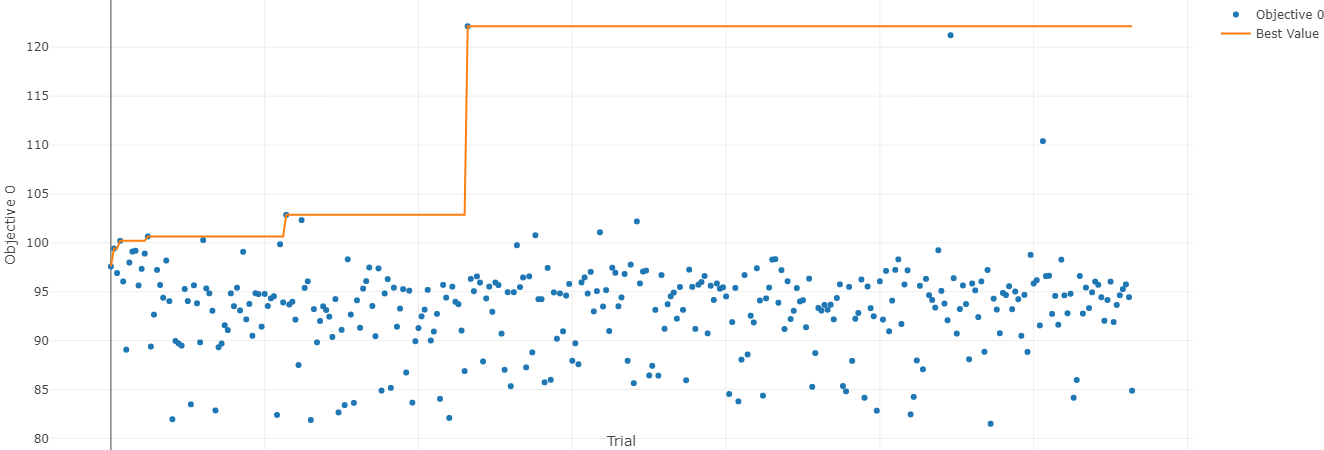
\includegraphics[width=14cm]{img/best_value.png}
    \caption{Best Value}
    \label{img:best_value}
    }
\end{figure*}

\begin{figure*}
\captionsetup{justification=centering}
\centering{
    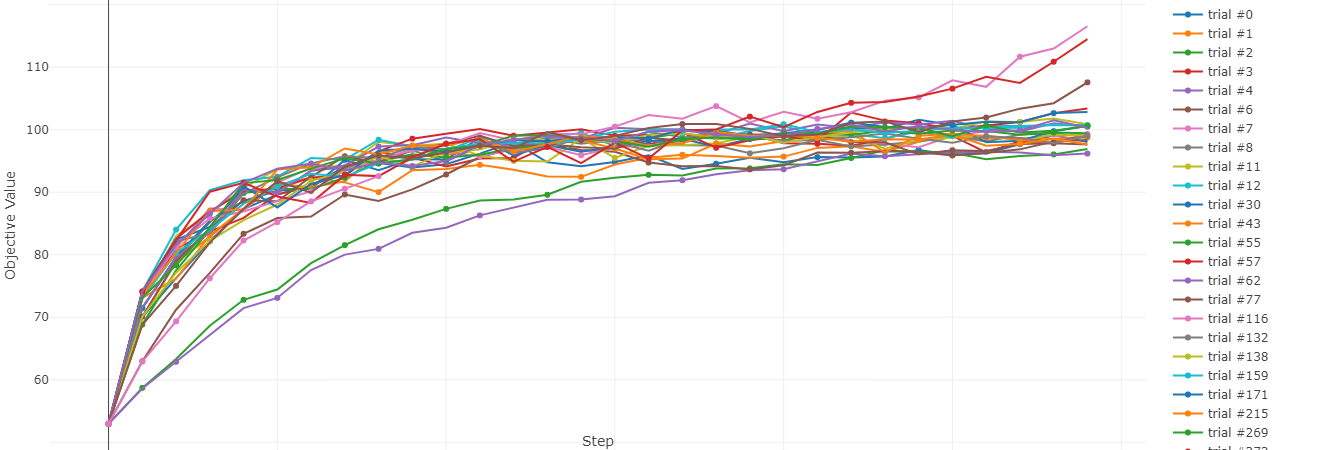
\includegraphics[width=14cm]{img/intermediate_value.png}
    \caption{Intermediate Value}
    \label{img:inter_value}
    }
\end{figure*}

\begin{figure*}[ht]
     \centering
    \begin{subfigure}[t]{0.85\textwidth}
        \raisebox{-\height}{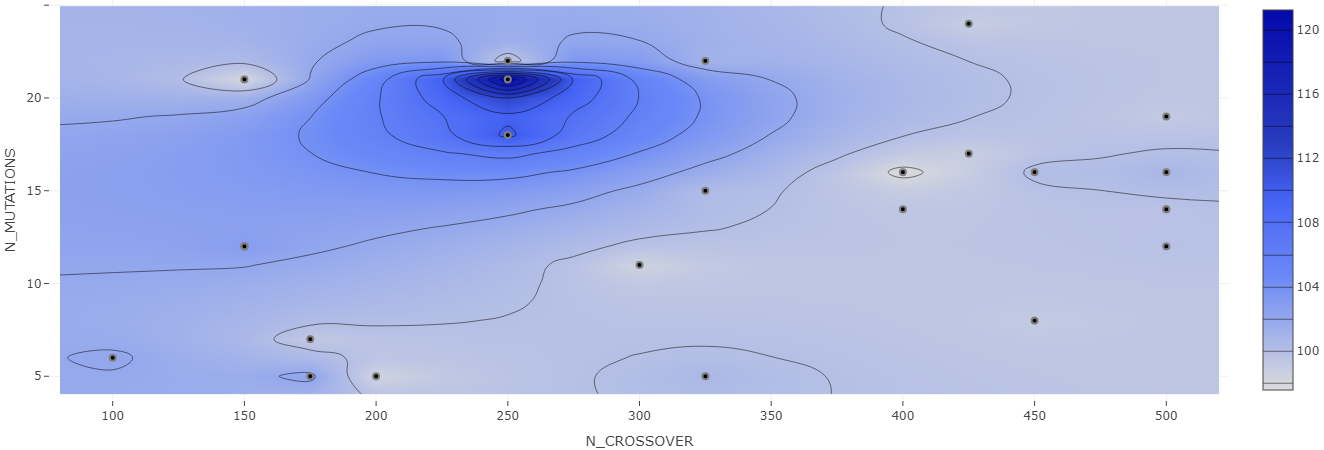
\includegraphics[width=\textwidth]{img/contour_mutn_cross.png}}
    \caption{Contour: N\_CROSSOVER and N\_MUTATION}
    \label{img:contour_cross_mutn}
    \end{subfigure}     
    \hfill
    \begin{subfigure}[t]{0.85\textwidth}
        \raisebox{-\height}{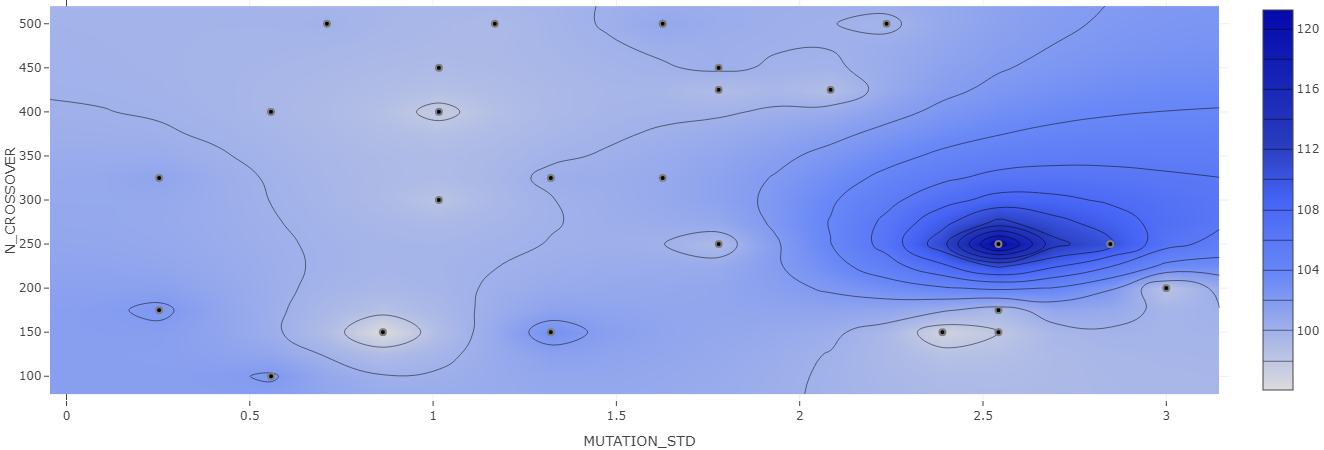
\includegraphics[width=\textwidth]{img/contour_mutstd_cross.png}}
    \caption{Contour: MUTATION\_STD and N\_CROSSOVER}
    \label{img:contour_mutstd_cross}
    \end{subfigure}
    \hfill
    \begin{subfigure}[t]{0.85\textwidth}
        \raisebox{-\height}{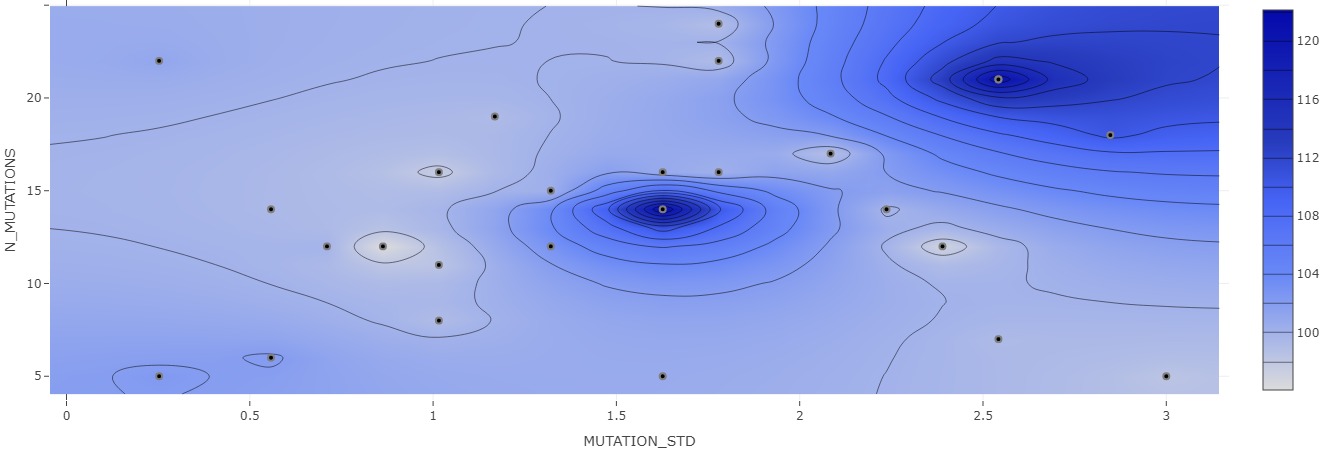
\includegraphics[width=\textwidth]{img/contour_mutstd_mutn.png}}
    \caption{Contour: MUTATION\_STD and N\_MUTATION}
    \label{img:contour_mutstd_mutn}
    \end{subfigure}
    \caption{Hyperparameter Contours}
    \label{img:hyper_contour}  
\end{figure*}




\begin{figure*}
\captionsetup{justification=centering}
\centering{
    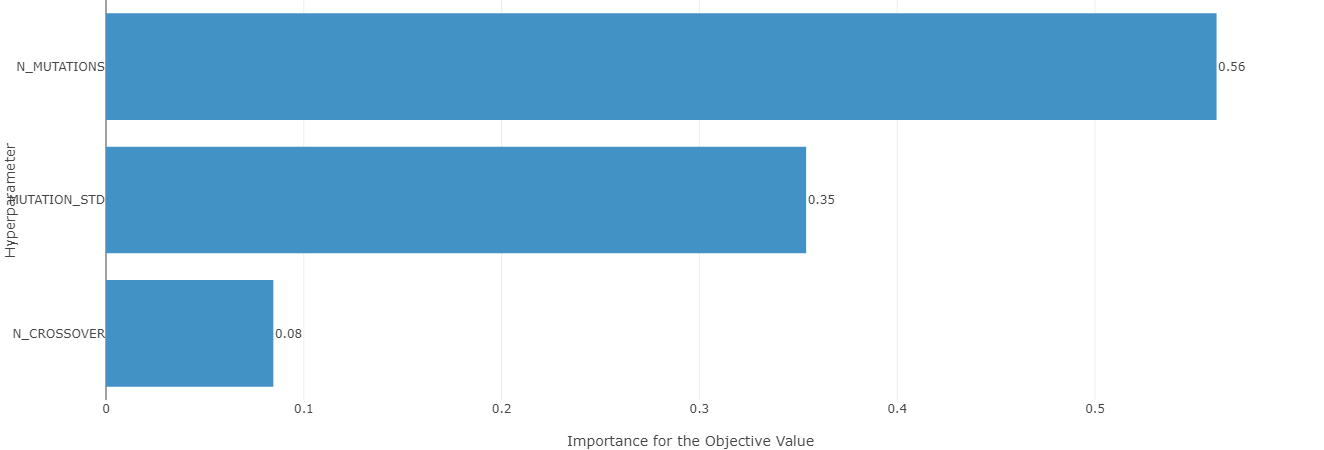
\includegraphics[width=14cm]{img/hyper.png}
    \caption{Hyperparameter Importance}
    \label{img:hyper}
    }
\end{figure*}

\section{Evaluation and Analysis} \label{evaluation}
In this section, we explored two ways to optimise our proposed model and analysed the effectiveness of these two optimisation strategies through evaluation results. We begin by analysing the results of hyperparameter optimisation in Section \ref{analyse_hyperparameters}. We then delve into the impact of changing language expressions on the model's performance in Section \ref{analyse_language}. 

\subsection{Analysis of Hyperparameter Optimisation} \label{analyse_hyperparameters}
Figure \ref{img:best_value} presents the objective value distribution for all the trials conducted during the optimisation process. From the graph, we can see that the majority of the trials resulted in objective values below 100, indicating poor performance. This could be due to several reasons such as the complexity of the problem or insufficient search space exploration. However, a few trials managed to achieve significantly higher objective values, leading to the production of a successful population with an average fitness score of over 120. This demonstrates the effectiveness of the optimisation process.

Figure \ref{img:inter_value} illustrates the trend of trials that improved the average fitness score over the course of 30 epochs. The y-axis represents the average fitness score, while the x-axis represents the number of epochs. From the graph, we can observe that the average fitness score generally increases for each trial. Furthermore, most trials experience significant growth in the earlier epochs, with some of them reaching peak performance in as few as 10 epochs. However, the rate of growth slows down in the later epochs, indicating that the population is converging towards an optimal solution. This trend is consistent with the principle of diminishing returns, where further improvements in performance become progressively more difficult to achieve as the system approaches an optimal state \cite{wiki:diminishing-returns}.

Based on the results shown in Figure \ref{img:hyper_contour}, it can be concluded that the optimal N\_CROSSOVER value is 250. Meanwhile, for the hyperparameters MUTATION\_STD and N\_MUTATION, the contour plot displays a local maximum at 1.5 standard deviation and 15 number of mutations, even though there is a global maximum at 2.5 standard deviation and 25 mutations. In addition to these findings, Optuna calculated the feature importance for the three hyperparameters, as shown in Figure \ref{img:hyper}. The results reveal that N\_MUTATION has the highest feature importance, with a weight of over 0.5, followed by MUTATION\_STD and N\_CROSSOVER. This indicates that N\_MUTATION plays a crucial role in optimising the performance of the genetic algorithm. However, it is essential to balance the number of mutations with the mutation standard deviation and the number of crossovers to achieve the best results. The contour plot in Figure \ref{img:hyper_contour} further supports this by showing that there is a clear optimal number of crossovers, while the optimal values for mutation standard deviation and the number of mutations have a local maximum. Thus, a balance must be found to maximize performance.

Based on the evaluation results, we can infer that the GA performed best with N\_CROSSOVER = 100, N\_MUTATION = 15, and MUTATION\_STD=5 for the change in constant value. However, it should be noted that 5 represents the maximum value within the hyperparameter range, indicating that the optimal standard deviation value may be higher. Overall, these findings suggest that the GA with the selected hyperparameters was effective in optimising the model.

\subsection{Analysis of Expanding Language Expression} \label{analyse_language}
Figure \ref{img:fitness_stats} depicts the impact of expanding the trigger expression on the GA's maximum and sum fitness scores. The maximum fitness of the population takes more time to converge to a single value after expanding the language expressions. Beforehand, it only took 5 epochs to reach an optimal solution, while after the expansion, 25 epochs were needed to reach an optimal solution. Moreover, the maximum fitness scores of the GAs after expression expansion are significantly greater than the scores before across all epochs. Before the expansion, the maximum fitness value goes from approximately 100 to 150, while after the expansion, it goes from just under 200 to 290.

In contrast, the sum fitness demonstrated a similar trend after expanding the language expression, but the overall amount decreased for each epoch. This is most likely due to the inclusion of more expressions in the trigger, making it more challenging for the GA to optimise the model, resulting in a lower sum fitness score. Further analysis is required to understand the impact of the expanded language expression on the GA's performance fully.

Overall, the evaluation results indicate that expanding the trigger expression with an additional clause leads to more optimal solutions. However, it also increases the optimisation difficulty, and therefore, there is a trade-off between optimisation difficulty and performance.

\begin{figure*}[ht]
     \centering
    \begin{subfigure}[t]{0.49\textwidth}
        \raisebox{-\height}{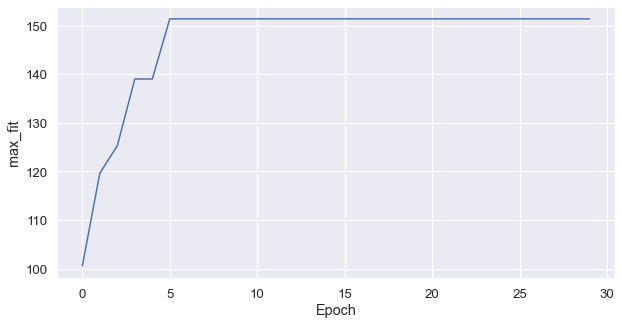
\includegraphics[width=\textwidth]{img/max_fit_before.png}}
    \caption{Maximum Fitness Trends Over Time}
    \label{img:max_fit_before}
    \end{subfigure}     
    \hfill
    \begin{subfigure}[t]{0.49\textwidth}
        \raisebox{-\height}{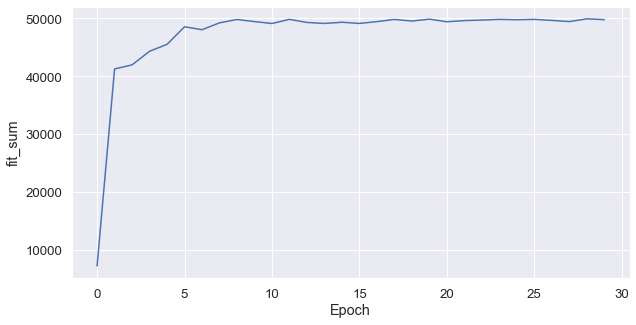
\includegraphics[width=\textwidth]{img/fit_sum_before.png}}
    \caption{Sum Fitness Trends Over Time}
    \label{img:fit_sum_before}
    \end{subfigure}
    \hfill
    \begin{subfigure}[t]{0.49\textwidth}
        \raisebox{-\height}{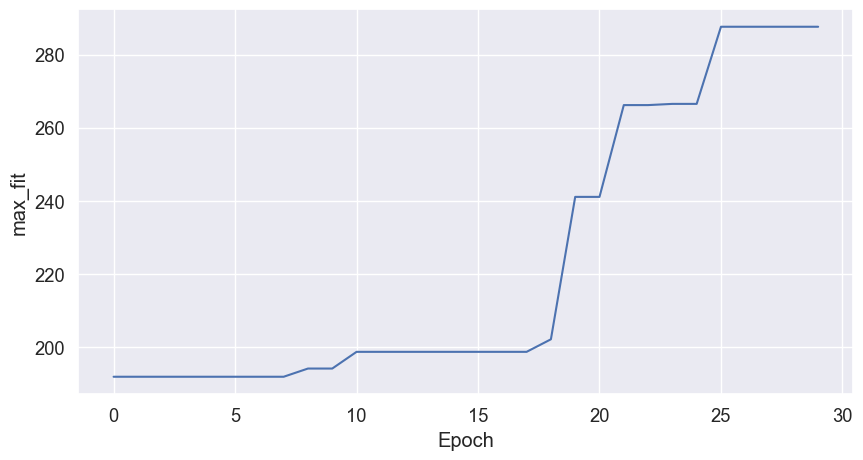
\includegraphics[width=\textwidth]{img/max_fit.png}}
    \caption{Maximum Fitness Trends Over Time After Expanding Expressions}
    \label{img:max_fit}
    \end{subfigure}
    \begin{subfigure}[t]{0.49\textwidth}
        \raisebox{-\height}{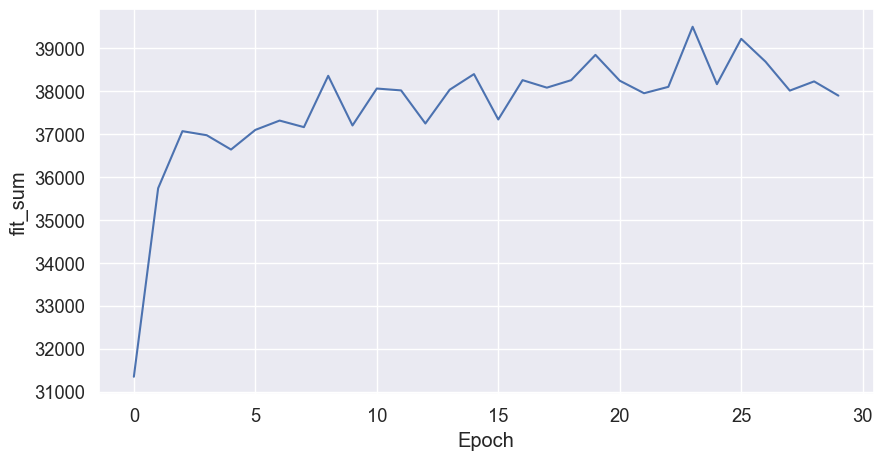
\includegraphics[width=\textwidth]{img/fit_sum.png}}
    \caption{Sum Fitness Trends Over Time After Expanding Expressions}
    \label{img:fit_sum}
    \end{subfigure}
    \caption{Fitness Statistics}
    \label{img:fitness_stats}  
\end{figure*}




\section{Conclusion} \label{conclusion}
This paper discusses an attempt to extend the GA presented by MacLachlan et al. by applying it to a trading bot optimisation framework. The framework focused on optimising the decision-making parameters of a Bitcoin trading bot using a GA by exploring a subset of the hypothesis space. The subset of the hypothesis space was defined by the expressiveness of the language that defined a candidate solution. 

The Optuna framework enabled grid-searching for the GA hyperparameters, with maximum fitness value being the evaluation metric. The hyperparameters being optimised included N\_CROSSOVER, N\_MUTATION, and MUTATION\_STD. Optuna's median pruner was used to terminate a trial if its performance is worse than the median of all other trials at a given epoch. Initial generations of GAs are seeded to allow the fair comparison of the different hyperparameter settings. 

The evaluation of the framework involved analysing indicators, candle values, and fitness metrics, such as maximum fitness and sum of fitness in the population. Using Optuna to explore the hypothesis space, the best set of hyperparameter values obtained for the GA were 100 crossovers, 15 mutations, and a standard deviation of 5 for the change in constant value. Notably, the optimal value for the standard deviation is expected to be higher than 5, as 5 represents the maximum value within the hyperparameter range. One conclusion that can be drawn from this is that the candidates might prefer coefficients that reduce the predicates to be only True or False which could be profitable in a market where the optimal decision is to, for example, buy early and sell at the end.

As the subset of the hypothesis space was restricted by the language defining a candidate solution the framework was limited as a more optimal solution could have been found beyond the confines of the language used. The model was also further limited by the use of default parameters for the indicators, indicators can only appear once in a given expression, and the format of a buy/sell trigger is limited to 4 expressions. Improvements to this model would address these limitations by defining a candidate solution with a less restrictive language. 

Further research and analysis could explore the hypothesis space even further by using different parameters for the indicators used and exploring a larger set of hyperparameters. A more robust analysis could be done by using multiple random initial generations for the GAs and optimising the framework based on the aggregate. 

\appendix
Word count: 2608

Links:
\begin{enumerate}
    \item\href{https://github.com/Kaiqi-Liang/CITS4404-Project}{GitHub Repository}
    \item\href{https://www.canva.com/design/DAFiUpjY3qA/PVPR4jqosqTpl8IfKcmbGA/view?utm_content=DAFiUpjY3qA&utm_campaign=designshare&utm_medium=link&utm_source=recording_view}{Canva Presentation}
\end{enumerate}

\bibliographystyle{IEEEtran}
\bibliography{reference}

\end{document}
